\documentclass{article}
\usepackage{ctex}

% Set page size and margins
% Replace `letterpaper' with `a4paper' for UK/EU standard size
\usepackage[letterpaper,top=2cm,bottom=2cm,left=2.5cm,right=2.5cm,marginparwidth=1.75cm]{geometry}

% Useful packages
\usepackage{amsmath}
\usepackage{graphicx}
\usepackage{subfigure}
\usepackage{float}
\usepackage[colorlinks=true, allcolors=blue]{hyperref}

\title{微分方程数值解计算实习课后作业12}
\author{陈文宇}
\date{\today}


\begin{document}


\maketitle

\tableofcontents

\newpage
%---------------------------------------------------
\section{实验结果}

下图是数值解和精确解的图像:
\begin{figure}[H]
\subfigure{
\begin{minipage}[t]{0.3\linewidth}
\centering
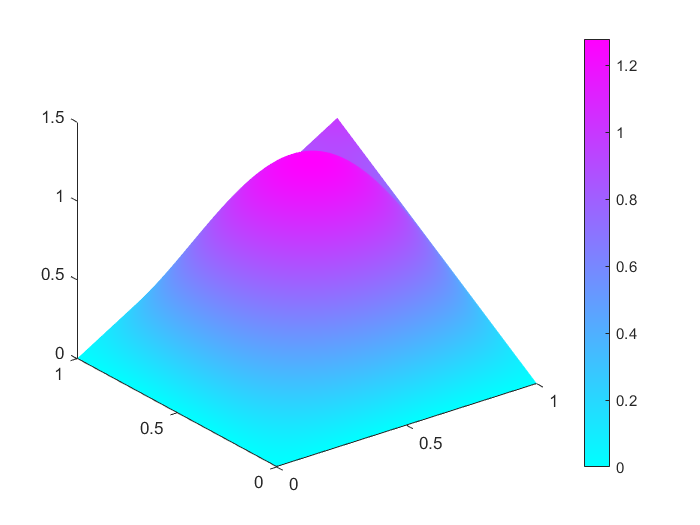
\includegraphics[scale=0.3]{solution_image.png}
\end{minipage}
}
\subfigure{
\begin{minipage}[t]{0.3\linewidth}
\centering
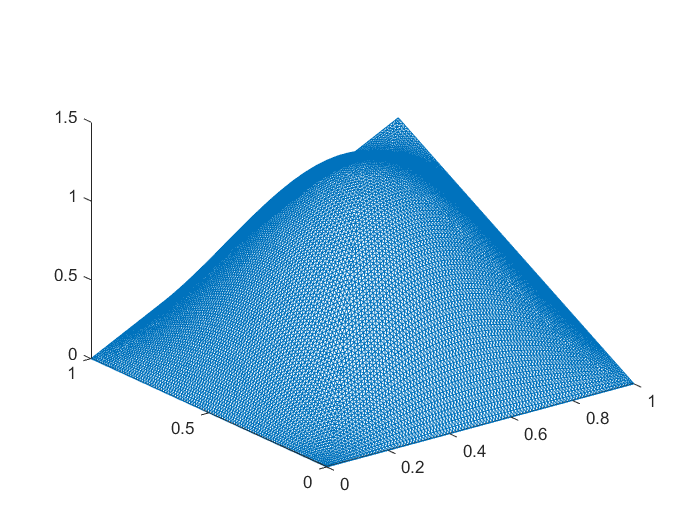
\includegraphics[scale=0.3]{solution_scatter.png}
\end{minipage}
}
\subfigure{
\begin{minipage}[t]{0.3\linewidth}
\centering
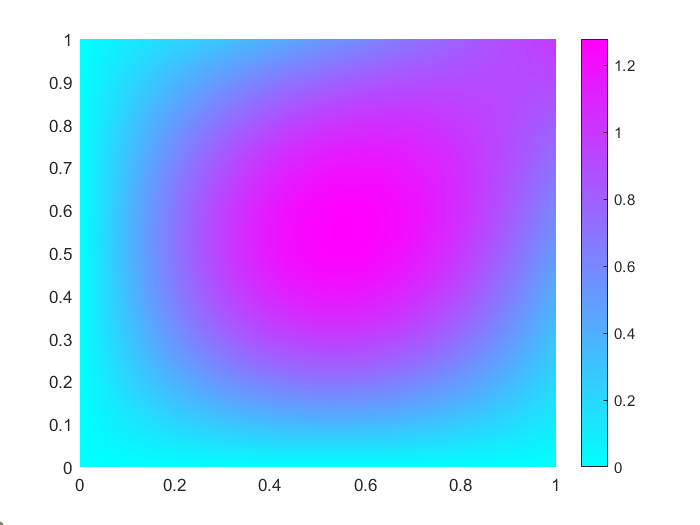
\includegraphics[scale=0.3]{solution_top.png}
\end{minipage}
}

\caption{\label{solution_image}数值解和精确解的图像}

\end{figure}

下图是$(logh,log(errC))$的图像,同$y=h^2$对比知,$errC$收敛阶为2.
\begin{figure}[H]
\centering
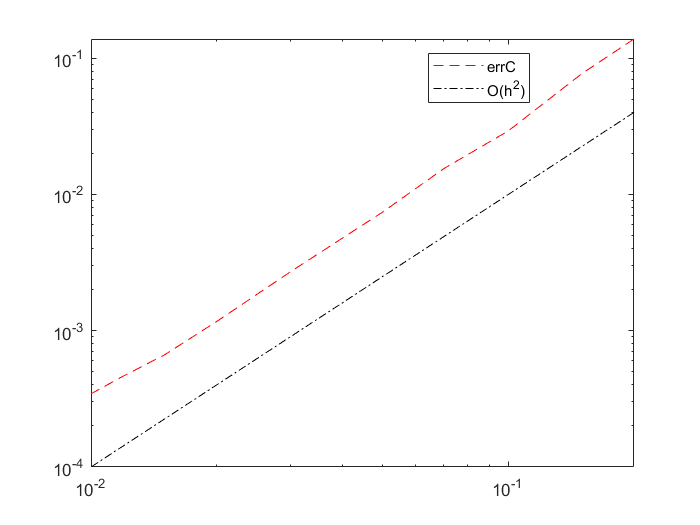
\includegraphics[scale=0.5]{errC.png}
\caption{\label{errC}$errC$ 误差的收敛阶}
\end{figure}

\newpage
下图是$(logh,log(err1))$的图像,根据线性基本拟合,知$err1$收敛阶为2.
\begin{figure}[H]
\centering
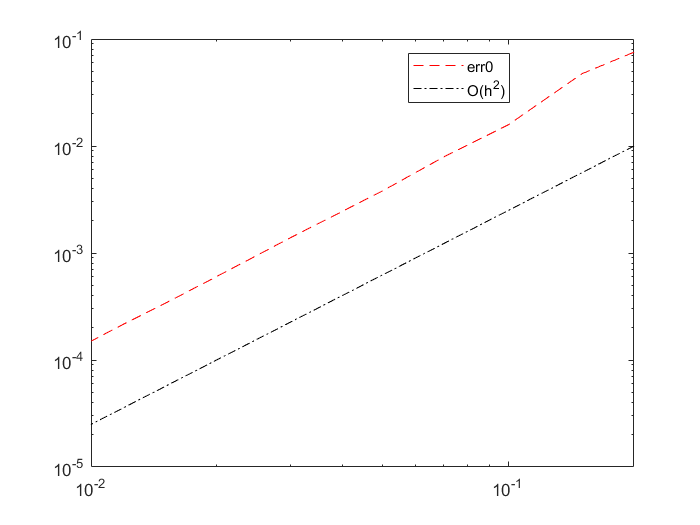
\includegraphics[scale=0.5]{err0.png}
\caption{\label{err0}$err0$ 误差的收敛阶}
\end{figure}

\begin{figure}[H]
	\centering
	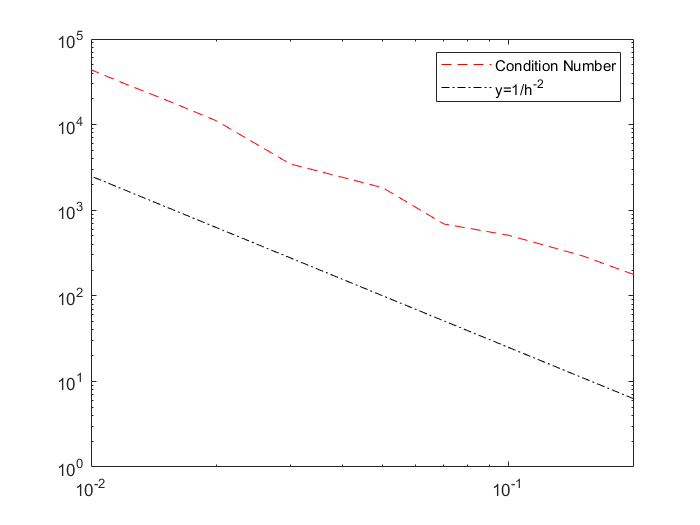
\includegraphics[scale=0.5]{CondN.png}
	\caption{\label{CondN}矩阵条件数}
\end{figure}


%-----------------------------------------------------
\section{实验结果分析}
对于本题,errC与err1误差的收敛阶为2
\end{document}